As noted in Section \ref{section: xshooter_ic5063: properties_of_outflowing_gas: uvb_vis_analysis_and_results: electron_temperatures}, the modelled values of the [OIII](5007/4363) and HeII$\lambda$4686/H$\beta$ ratios depend on the electron density and metallicity of the emitting gas, the spectral index of the AGN continuum, and the ionisation parameter. In order to investigate the impact of this on ionisation-mechanism diagnostics, I present photoionisation models with varied values of these parameters here. The principal goal of this analysis is to determine if there exists a reasonable set of parameters which can explain the measured ratios for IC\;5063 (Chapter \ref{chapter: xshooter_ic5063}; Figure \ref{fig: xshooter_ic5063: heii_hbeta}) as being entirely due to AGN photoionisation, which would remove the need to include a contribution from shocks.

The $\textsc{Cloudy}$ photoionisation code was used for this purpose. The models were set up in the same way as described in Sections \ref{section: xshooter_ic5063: properties_of_outflowing_gas: uvb_vis_analysis_and_results: transauroral_lines} and  \ref{section: stis_seyferts: tr_diagnostics}, in which they were used to produce grids for the transauroral-line ratios. Single-slab, plane-parallel, radiation-bounded models of dust-free photoionised gas with an electron density of $n_e=10^3$\;cm$^{-3}$ were produced for varying metallicities, spectral indices and ionisation parameters.

In Figure \ref{fig: heii_hb_oiii_photoionisation_modelling: heii_hbeta_alpha} the modelled ratios for a solar-composition gas of density $n_e=10^3$\;cm$^{-3}$ with three different spectral indices of the AGN-photoionising continuum ($\alpha = 1.0, 1.5$, and $2.0$; each marked with different symbols) and ionisation parameters ranging between \mbox{$-3.0$\;\textless\;log$_{10}U$ \textless\;$-1.5$} are presented. It can be seen that varying the ionisation parameter for a given spectral index can change the [OIII](5007/4363) ratio by a factor of two, while the effect on the HeII$\lambda$4686/H$\mathrm{\beta}$ ratio is only a factor of $\sim$1.25 in the most extreme case. Changing the spectral index has a similar effect on the [OIII] ratio: the modelled ratio for $\alpha=1.5$ is a factor of $\sim$1.5 higher than for $\alpha=1.0$. Furthermore, the chosen spectral index also has a non-negligible effect on the HeII$\lambda$4686/H$\mathrm{\beta}$ ratio, with the ratio for $\alpha=1.5$ being a factor of $\sim$1.5 higher than for $\alpha=1.0$.

The variation in the modelled ratios for $\alpha=1.5$ with gas metallicities ranging from 0.5--2.0\;$Z_\odot$ is shown in Figure \ref{fig: heii_hb_oiii_photoionisation_modelling: heii_hbeta_z}, with higher metallicities having larger marker sizes. As with spectral index and ionisation parameter, the chosen gas metallicity also has a significant effect on the modelled [OIII] ratio, however, the effect on HeII$\lambda$4686/H$\mathrm{\beta}$ is negligible. Finally, I investigate the effect that electron density has on the modelled ratios by fixing the ionisation parameter to log$U=-2.75$ for a solar-metallicity gas with three spectral indices ($\alpha=1.0, 1.5$, and $2.0$), and varying the electron density between \mbox{2.0\;\textless\;log$_\mathrm{10}$($n_e$\;[cm$^{-3}$])\;\textless\;5.0}, as is shown in Figure \ref{fig: heii_hb_oiii_photoionisation_modelling: heii_hbeta_ne}.

Given the ratios that are measured from the apertures of the outflowing regions in IC\;5063 (Chapter \ref{chapter: xshooter_ic5063}, Figure \ref{fig: xshooter_ic5063: heii_hbeta}), it is found that for $\alpha=1.5$, only metal-poor gas ($\sim$0.5\;$Z_\odot$), a higher electron density than is measured ($n_e$\;\textgreater\;$10^{3.5}$\;cm$^{-3}$; Section \ref{section: xshooter_ic5063: properties_of_outflowing_gas: uvb_vis_analysis_and_results: transauroral_lines}), and a much higher ionisation parameter can explain the observed ratios as being solely due to AGN photoionisation. The gas mass contained in the disk of IC\;5063 is $M_\mathrm{disk}\gtrapprox 1 \times 10^9$\;M$_\odot$ (from the molecular phase; \citealt{Morganti2015}), corresponding to an approximate stellar mass of $M_*\sim10^9$\;M$_\odot$ \citep{Maddox2015}, which would imply a metallicity of $12+\mathrm{log(O/H)}\approx8.6$ using the relation given by \citet{Tremonti2004}. A metallicity of 0.5\;Z$_\odot$ corresponds to $12+\mathrm{log(O/H)}\approx8.3$, lower than would be expected for IC\;5063 given the mass of its disk. 

However, the spectral index of $\alpha=1.5$ is an assumption --- it is feasible that some combination of ionisation parameter (which varies between kinematic components), along with a different spectral index, can produce line ratios similar to those found for the warm-ionised gas in IC\;5063 without the need for an additional shock component.

\begin{figure}
    \begin{subfigure}[t]{0.49\textwidth}
        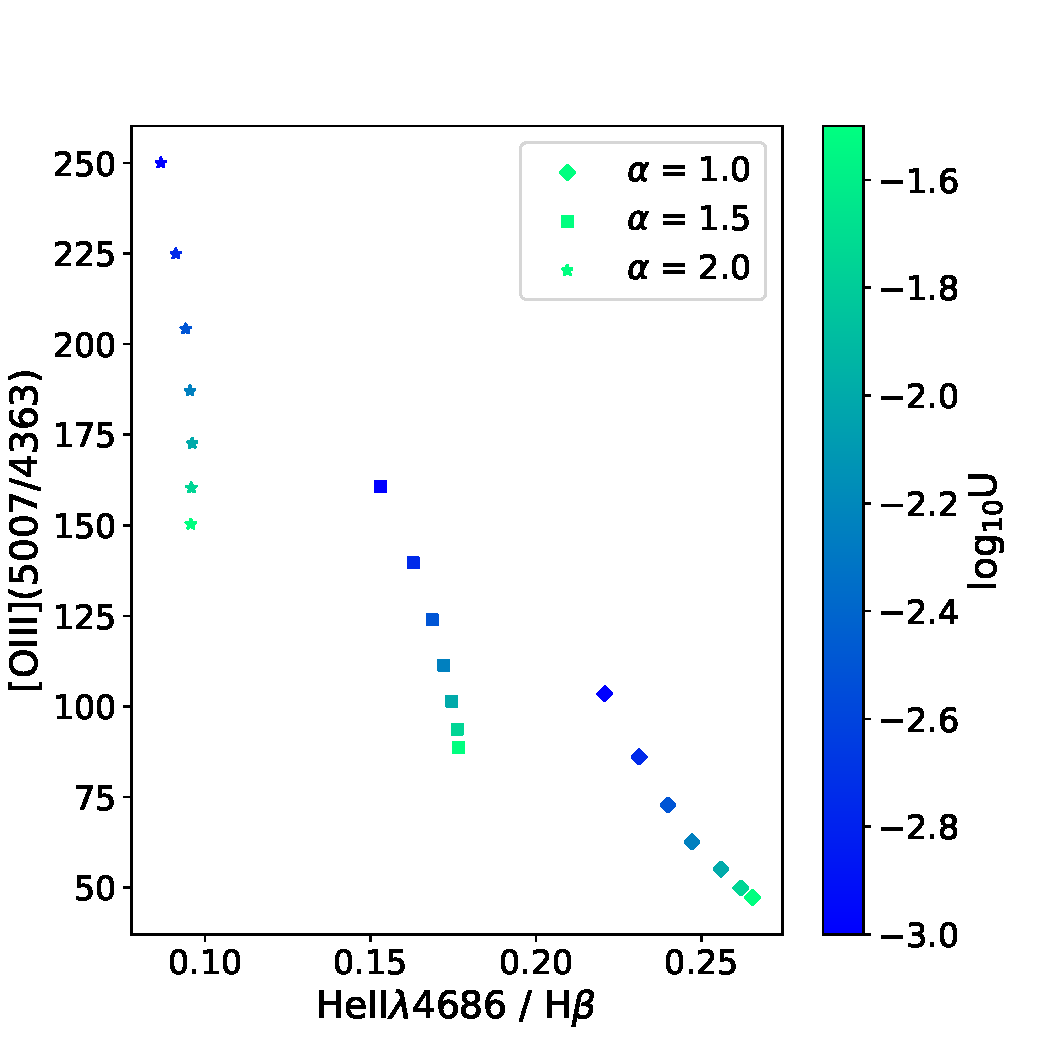
\includegraphics[width = \linewidth]{figures/heii_hb_oiii_photoionisation_modelling/3ne_a_vary_10z.pdf}
        \captionsetup{width=.9\linewidth}
        \caption{Modelled line ratios for a gas density of $n_e=10^3$\;cm$^{-3}$ and an ionising source of varying spectral index and ionisation parameter. Spectral indices of $\alpha=1.0, 1.5$, and $2.0$ are shown by diamonds, squares and stars respectively.}
        \label{fig: heii_hb_oiii_photoionisation_modelling: heii_hbeta_alpha}
    \end{subfigure}
    \hfill
    \begin{subfigure}[t]{0.49\textwidth}
        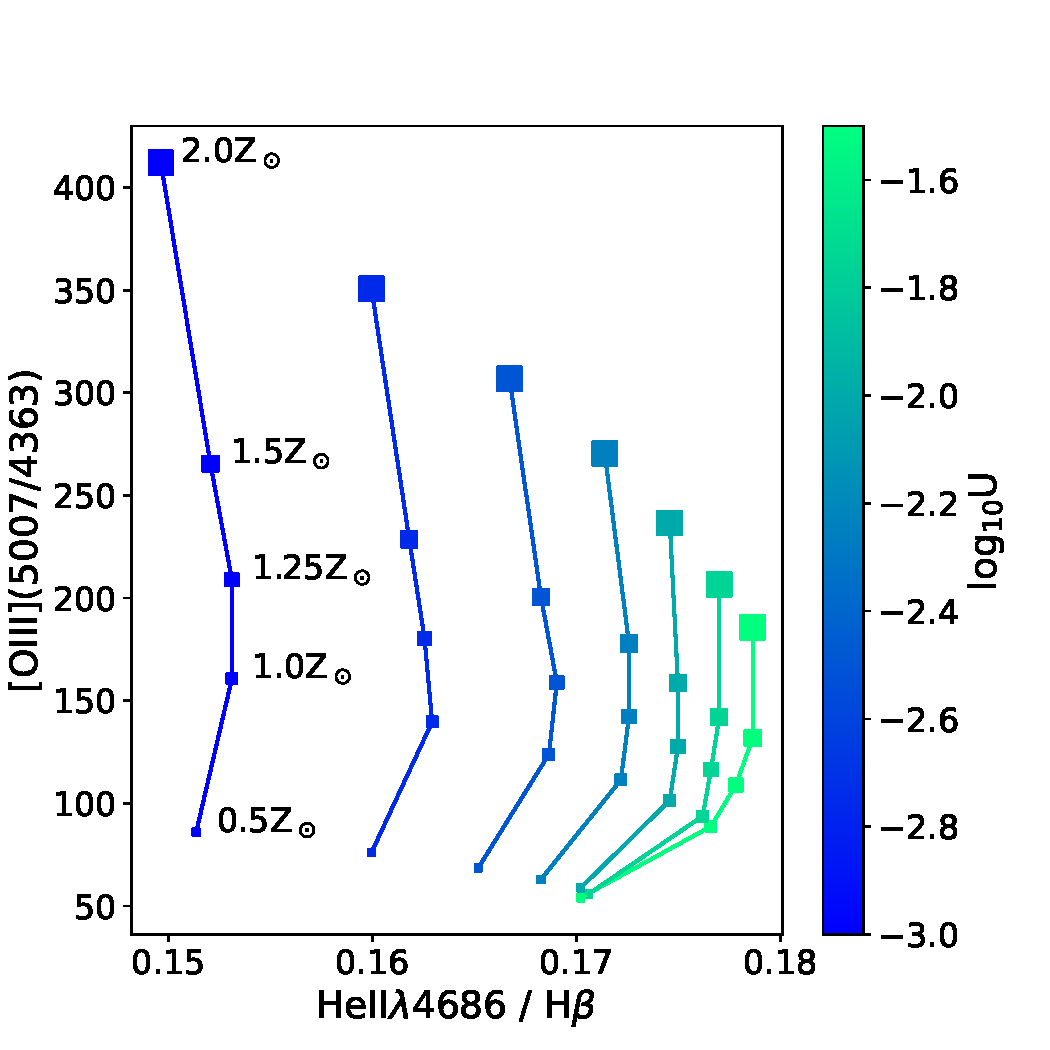
\includegraphics[width = \linewidth]{figures/heii_hb_oiii_photoionisation_modelling/3ne_15a_z_vary.pdf}
        \captionsetup{width=.9\linewidth}
        \caption{Modelled line ratios for $\alpha=1.5$ and varying metallicities. The different fractions of solar abundance, ranging from 0.5--2\;$Z_\odot$ in steps of 0.5\;$Z_\odot$, are shown with different marker sizes (labelled). Points with the same ionisation parameter are joined to show the variation with metallicity.}
        \label{fig: heii_hb_oiii_photoionisation_modelling: heii_hbeta_z}
    \end{subfigure} \\
    \vfill
    \centering
    \begin{subfigure}[t]{0.49\textwidth}
        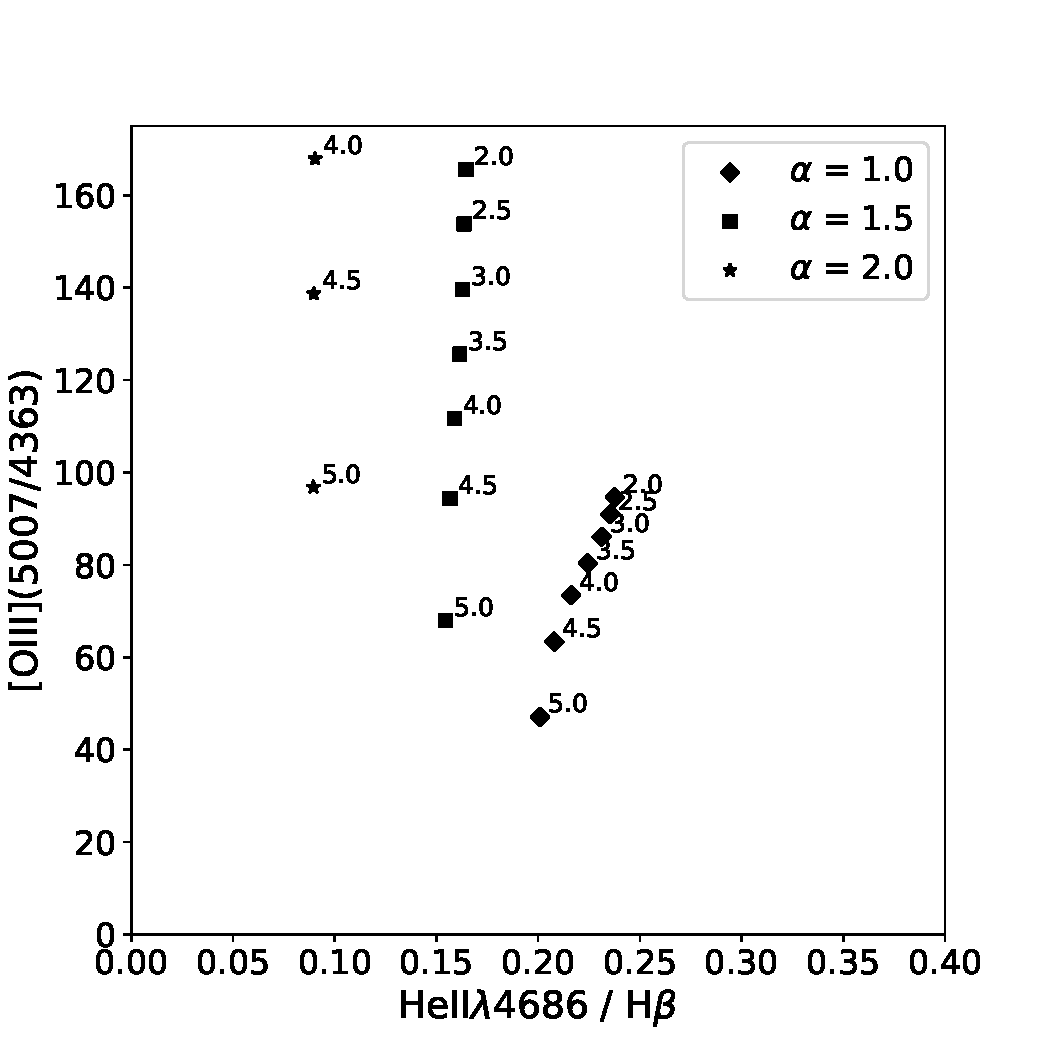
\includegraphics[width = \linewidth]{figures/heii_hb_oiii_photoionisation_modelling/ne_vary.pdf}
        \caption{Modelled line ratios for log$U=-2.75$ and varying electron densities in the range \mbox{2.0\;\textless\;log$_\mathrm{10}(n_e$\;[cm$^{-3}$])\;\textless\;5.0} (labelled).}
        \label{fig: heii_hb_oiii_photoionisation_modelling: heii_hbeta_ne}
    \end{subfigure}
    \vspace{0.2cm}
    \caption[The HeII$\lambda$4686/H$\mathrm{\beta}$ vs {[}OIII{]}$\lambda$5007/4363 diagnostic diagram with varying model parameters.]{HeII$\lambda$4686/H$\mathrm{\beta}$ vs [OIII]$\lambda$5007/4363 line ratios from photoionisation modelling of a solar-composition gas with plane-parallel geometry and varying model parameters. In the top two panels, the variation in ionisation parameter is shown by the colour bar (ranging between \mbox{$-3.0$\;\textless\;log$_{10}U$\;\textless\;$-1.5$} in steps of 0.25). Note that the axis limits are different than those used in Figure \ref{fig: xshooter_ic5063: heii_hbeta}.}
\end{figure}